\documentclass[%
a4paper,
%twoside,
11pt
]{article}

% encoding, font, language
\usepackage[T1]{fontenc}
\usepackage[utf8]{inputenc}
\usepackage{lmodern}
\usepackage[english]{babel}

\usepackage{nicefrac}

\usepackage[
    % handwritten,
    nowarnings,
    %myconfig
]
{xcookybooky}

\DeclareRobustCommand{\textcelcius}{\ensuremath{^{\circ}\mathrm{C}}}


\setcounter{secnumdepth}{1}
\renewcommand*{\recipesection}[2][]
{%
    \subsection[#1]{#2}
}
\renewcommand{\subsectionmark}[1]
{% no implementation to display the section name instead
}


\usepackage{hyperref}    % must be the last package
\hypersetup{%
    pdfauthor            = {Magdalena Przybyła, Hubert Bereś},
    pdftitle             = {Bethan and Hugh's cookbook},
    pdfstartview         = {FitV},
    pdfview              = {FitH},
    pdfpagemode          = {UseNone}, % Options; UseNone, UseOutlines
    bookmarksopen        = {true},
    pdfpagetransition    = {Glitter},
    colorlinks           = {true},
    linkcolor            = {black},
    urlcolor             = {blue},
    citecolor            = {black},
    filecolor            = {black},
}

\hbadness=10000	% Ignore underfull boxes

\usepackage{graphicx}
\graphicspath{ {./pic/} }

\begin{document}

\title{Bethan and Hugh's cookbook}
\author{Magdalena Przybyła, Hubert Bereś}
\maketitle

\begin{abstract}
    Some initial blah blah.
\end{abstract}

\tableofcontents

\vspace{5em}
\newpage

\section{Breakfast}

% Complete recipe example
\begin{recipe}
[% 
    preparationtime = {\unit[15]{min}},
    bakingtime={\unit[50]{min}}
]
{Banana bread with blueberries}
 \introduction{%
	Forgot about bananas? This recipe will save them. Perfect for afternoon tea or even breakfast. Simple sweet treat!  
}

    \ingredients{%
    	4-5 & Ripe bananas \\
        0.25 c. & Oil \\
        0.25 c. & Peanut butter \\
        0.25 c. & Milk \\
        2 handf. & Blueberries (fresh or frozen) \\
        & \\
        2 c. & Flour \\
        0.5 c. & Sugar \\
        1.5 ts. & Baking powder \\
        2 handf. & Desiccated coconut \\
        1 handf. & Chopped nuts \\
        & Spices (cinnamon, ginger, cardamom)
       }

    \preparation{%
       \step Turn bananas into purée (blend or use fork), mix with all other 'wet' ingredients. 
       \step Mix all dry ingredients in a separate bowl. Add in small portions and mix into the wet ingredients.
       \step Add blueberries.
       \step Bake for about 50 min at \unit[180]{\textcelcius} in a small rectangular tin lined with baking paper.
    }

 \hint{%
	You can skip blueberries and add some chocolate chips.
}

\end{recipe}
\newpage
\begin{recipe}
    [%
        preparationtime = {\unit[5]{min}},
        portion = {\portion{3-4}},
        bakingtime = {\unit[10-15]{min}}
    ]
    {Polish apple crumpets}
    \introduction{%
        This recipe encourages you to explore apples: you need to take an account on their tenderness - the more crisp and firm apple, the thinner the slices! How many kinds of apples do you know? Granny Smith doesn't count, if I had power, I would erase it!

        PS You don't need muffin rings, in Poland we actually prefer crumpets to be uneven and more oval.
    }

    \ingredients{%
        4 & Apples (big) \\
        1.5 c. & Milk \\
        1.5 c. & Flour \\
        3 tbs. & Sugar \\
        1 ts. & Baking powder/soda
    }

    \preparation{%
        \step Mix well all the batter ingredients.
        \step Cut apples into 0.5-1cm heigh slices (remove cores).
        \step Dig apple slices in the batter and fry.
        \step Serve with caster sugar or confiture.
    }

    \hint{%
        I prefer to leave apple skin but you can peel it, especially if you use 'allotment apples' or some of the so called 'old kind' such as reinette.
    }

\end{recipe}
\newpage
\begin{recipe}
    [% 
        preparationtime = {\unit[15]{min}},
        bakingtime = {\unit[30]{min}}
    ]
    {Granola}

    \introduction{%
        There's nothing better than a quick home-made breakfast. Granola is a great base - add seasonal fruit, yoghurt or milk and bob's your uncle, delicious meal is ready.
    }

    \ingredients{%
        2.5 c. & Regular rolled oats \\
        0.5 c. & Walnuts \\
        0.5 c. & Hazelnuts \\
        0.5 c. & Sunflower seeds \\
        0.5 c. & Honey \\
        0.25 c. & Oil \\
        2 ts. & Cinnamon \\
        2 ts. & Ginger \\
        Pinch & Salt
    }

    \preparation{%
        \step Heat honey and oil slightly, just so you can mix them. Add spices and salt.
        \step In a big bowl, mix oats and nuts. Add honey/oil mixture and cover everything evenly.
        \step Transfer granola to big and flat baking tray, spread out evenly. \underline{Bake at  \unit[180]{\textcelcius} for 20-30 min}, mix with spatula every 5 min and keep an eye not to burn the granola!
        \step Store in an airtight jar.
    }

    \hint{%
        When the granola cooled down, you can add chopped dried fruit - eg. apricots and cranberry. You can also add some coca powder to honey - this granola will be happy when accompanied by dried cherries. Use different flakes (check out millet flakes or barley flakes - you can find them in polish shops certainly). You can also add some orange juice to honey. Chocolate chips, coconut flakes, etc...  There's so much room for imagination!
    }

\end{recipe}
\newpage
% Complete recipe example
\begin{recipe}
[% 
    preparationtime = {\unit[5]{min}},
    portion = {\portion{1}},
    bakingtime={\unit[10]{min}}
]
{Omelette}
 \introduction{%
This recipe is for one serving. However you can double the ingredients and make one, big omelette for more people (can be tricky to fry, though). What I usually do: instead of 'omelette batch' I prepare simultaneously two omelettes (or more) - two bowls with beaten eggs, two frying pans, etc... 
}

    \ingredients{%
    	2-3 & Eggs \\
    	0.25 c. & Milk \\
    	Handf. & Spinach \\
    	30 g & Feta cheese \\
    	5 & Cherry tomatoes \\
    	5 & Olives \\
    	Handf. & Grated cheddar \\
    	 & Smoked paprica \\
    	& Salt\&pepper \\
    	& Butter to fry 
        }

    \preparation{%
       \step Beat eggs, add milk, salt\&pepper and mix again.
       \step On preheated frying pan melt butter and pour egg mixture. Let is settle for 30s, mix gently not congealed part (don't disturb the bottom layer!). Immediately add all toppings and stir them in. Sprinkle with smoked paprika
       \step After 1 min, turn down the heat. Cover with lid. After 2-3 min fold the omelette in half, add a little bit of boiling water on the pan and cover with lid (create steam so inner part of the omelette can cook quicker). 
       \step After 2-3 min, sprinkle with smoked paprika, turn (if possible) for extra 30s. The omelette is done!
    }

 \hint{%
Instead of folding and playing with steam, you can simply turn the omelette and fold it after cooking.
}

\end{recipe}
\newpage
\begin{recipe}
    [% 
        preparationtime = {\unit[5]{min}},
        bakingtime={\unit[10]{min}}
    ]
    {Orange dessert sauce}
    \introduction{%
        ***proportions are rough***

        Crepes (with curd cheese), ice cream, fondée... or straight from the pot! This sauce serves as a cherry on top
    }

    \ingredients{%
        \unit[100-150]{g} & Butter \\
        0.5-1 c. & Cane sugar \\
        3 & Oranges
    }

    \preparation{%
        \step In a deep frying pan or a pot with big diameter, melt butter.
        \step Add orange juice and sugar. Simmer (so that you can observe small bubbles), without a lid, for 10 to 15 min.
    }

    \suggestion
    {%
        As this sauce is based on fat and sugar, and ideally all water evaporates during simmering, it can get dangerously hot. A minute of reheating in the microwave and the tupperware has melted...
    }

    \hint{%
        Sauce thickens as it cools down. However, if you suspect it's too running, add more sugar.
    }

\end{recipe}
\newpage
\begin{recipe}
    [% 
        preparationtime = {\unit[15]{min}},
        portion = {\portion{2}},
        bakingtime = {\unit[15]{min}}
    ]
    {Fruity omelette}

    \ingredients{%
        5 & Egg \\
        \nicefrac{1}{2} c. & Flour \\
        1 ts. & Baking powder \\
        \nicefrac{1}{4} c. & Sugar \\
        \nicefrac{1}{4} c. & Milk/water \\
        & Raspberries \\
        \nicefrac{1}{2} c. & Yoghurt/quark to serve with
    }

    \preparation{%
        \step Beat eggs with milk.
        Mix well with flour, baking powder and sugar.
        \step Gently stir raspberries in.
        \step Pour the mixture on a preheated frying pan.
        \step Fry for 4 min on medium heat, after that cover the pan and leave for another 4 min.
        \step Flip the omelette and repeat step 4.
        \step Serve with yoghurt, honey, nuts... whatever you fancy!

    }

    \hint{%
        You can also add a little bit of yoghurt or quark to the batter, as weel as some spices - ginger, cinnamon...
    }

\end{recipe}
\newpage

\section{Lunch}

\begin{recipe}
    [% 
        preparationtime = {\unit[10]{min}},
        portion = {\portion{2}},
        bakingtime = {\unit[15]{min}}
    ]
    {Broccoli pesto}

    \introduction{%
        My grandma who cooks only traditional food fell in love in this pesto.
        I can recommend it more!
    }

    % \setRecipeLengths{
    %     ingredientswidth=10cm
    % }
    % TODO: Magda: ingredient names should be short.
    % Please move processing descriptions like chopping or pressing to the actual recipe.
    % This looks better and is easier to format.
    % The above command tweaks width of the ingredients pane.

    \ingredients[13]{%
        1 & Broccoli with stem \\
        \unit[0.75]{c.} & Olive oil \\
        \unit[1]{c.} & Roasted almond (or sunflower seeds) \\
        4-5 & Garlic cloves \\
        1 & Onion, diced \\
        2cm & Ginger, diced \\
        3 & Garlic cloves, diced/pressed \\
        0.5 bunch & Parsley \\
        \unit[5]{tsp} & \underline{Yeast flakes} \\
        & Chili \\
        & Nutmeg \\
        & Lemon juice \\
        & salt\&pepper
    }

    \preparation{%
        \step Cut broccoli into pieces, cook on boiling water for 4-5 min.
        Drain and cool with cold water (preserve nice green colour).
        \step Blend everything.
        \step Voilà!
    }

    \suggestion{%
        Serve with pasta, topped with cheese and cherry tomatoes.
        Or serve with bread.
        Or even with roast (as sauce) or raw vegetables (as dip).
    }

    \hint{%
        To roast almonds (or any other seeds/nuts), preheat the frying pan well (the thicker the frying pan, the better (eg cast-iron)), do not add any fat.
        Keep it at high heat, stir from time to time (not too often, though!
        Let them roast).
        Remember to transfer them immediately to a bowl/suitable tupperware as the frying pan is still hot after turning the hob off.
    }

\end{recipe}
\newpage
% Complete recipe example
\begin{recipe}
[% 
    preparationtime = {\unit[15]{min}},
    portion = {\portion{4}},
    bakingtime={\unit[25]{min}}
]
{Ratatouille or lecsó}
 \introduction{%
 	When first courgettes appear in the allotment is time for lecsó (and then for courgette ketchup but this is a story for another time). 
 	
	Our arbitrary decision was to call lecsó 'ratatouille with meat', so this is the distinction....If you want lecsó then, add fried sausage at the end of cooking ratatouille ;)
	
	Smoked paprika is \underline{essential}, all the taste is hidden here. 
	
	If you can find one, exchange some of the courgettes for a marrow but remember, that marrow usually requires peeling. 
}

    \ingredients{%
    	4 & Courgettes \\
        3  & Sweet longitudinal peppers \\
        1 & Red onion \\
        2 c. & Tomatoes \\
        2 tbs. & Smoked paprika \\
        2 tbs. & Paprika \\
        1 ts. & Hot paprika \\
        1 tbs. & Sugar 
       }

    \preparation{%
       \step Dice onion, fry with all spices. Add peppers (big squares) and courgettes (quarter moons) and fry for 5 min.
       \step Add tomatoes, add salt to taste, and cook for 5-8 min.
       \step Add fried sausage or chickpea. 
       \step Serve with crusty bread.
    }

 \hint{%
	You can also add aubergines but as they need more time to cook, fry them for extra 4 min before adding other vegetables. There's also a creamy version available - add marrow, exchange peppers for carrots, reduce amount of smoked paprika, add cream and fresh herbs (eg. parsley or... lovage).
}

\end{recipe}
\newpage
\begin{recipe}
    [% 
        preparationtime = {\unit[30]{min}},
        portion = {\portion{4}},
        source = {Fridge leftovers improvisation}
    ]
    {Green lentil wraps}

    \ingredients{%
        8 & tortillas (wholemeal) \\
        \unit[100]{g} & green lentils \\
        1 & green pepper \\
        1 & onion \\
        & green beans \\
        & salad mix \\
        & green peas or mangout \\
        & grated cheese \\
        & salsa sauce
    }

    \preparation{%
        \step Boil the lentils until soft with roughly three times as much water (add some salt).
        Boil the green peas in another pan.
        \step Fry the onion and pepper on medium fire.
        \step Prepare a large, dry and clean, non-stick frying pan and keep it on minimum heat.
        On a flat surface mix all the ingredient on a tortilla and roll.
        To keep your fingers clean put the salsa at the bottom and the salad at the top.
        \step Fry the wraps, turning by 90 degrees when they become brown and stiff.
    }

    \suggestion[Rolling a wrap]
    {%
        Put the filling only on the bottom half, leaving \unit[2-3]{cm} margin on the sides.
        With both hands fold around 1/6 of perimeter on each side,
        % TODO: 1/6
        leaving another 1/6 at the bottom.
        Now holding the sides and pushing them to the middle as you go, roll the bottom over the top.
        Don't be afraid to compress the ingredients.
    }

    \hint{%
        While frying start with the place where the layers meet.
        Then turn as if you continued to roll it rather than unrolling on the pan!
    }
\end{recipe}
\newpage

\begin{recipe}
[% 
    preparationtime = {\unit[0.5]{h}},
    bakingtime={\unit[0.5]{h}},
     portion = {\portion{4}}
]
{Risotto}
    
    \introduction{%
    	People still haven't figured out why exactly stirring makes risotto so delicious. There are a few theories, covering even spread of heat and increased 'leakage' of starch from rice grains. Regardless of the reason, bear in mind that stirring, keeping the broth hot at all time and adding it in small portions are essential! 
    }
    
    \ingredients{%
        350 g  & Risotto rice \\
        Bunch  & Asparagus \\
        3 & Red/yellow peppers \\
        1 & Red onion \\
        500 ml & Broth/stock \\
        200 ml& Apple cider \\
        & Cheese (Parmesan or mature cheddar) \\
        250 g & Pancetta (Smoked) 
    }
    
    \preparation{%
        \step Heat up broth and keep hot.
        \step Fry finely diced onion. Add rice and fry for 2-3 minutes.
        \step Add alternately broth and cider in small portions (ladle or two) at a time. Keep stirring rice. Add more liquid when previous portion almost absorbed. 
        \step In meantime roast peppers and fry asparagus (cut in 3 pieces) or fry both. Fry pancetta.
        \step Stir vegetable and pancetta in. Add cheese. 
       
    }
    
    \suggestion[]
    {%
      The larger the pan, the less stirring required as rice is heated more evenly. 
    }
    
\end{recipe}
\newpage
\begin{recipe}
    [% 
        preparationtime = {\unit[10]{min}},
        portion = {\portion{2-4}},
        bakingtime = {\unit[30]{min}}
    ]
    {Roast cauliflower and chickpea lunch}

    \introduction{%
        Roast vegetables, spices and pulses - the quickest lunch ever!
        This roast can be served alone but to make it more filling you can add some grains or baguette.
    }

    \ingredients{%
        1 & Cauliflower \\
        1 can & Chickpea \\
        250 g & Cherry tomatoes \\
        &  \\
        3 tbs. & Oil \\
        2 tbs. & Soy sauce \\
        1 tbs. & Vinegar \\
        1 tbs. & Honey \\
        1 tbs. & Smoked paprika \\
        1 ts. & Hot paprika \\
        1 ts. & Coriander \\
        1 ts. & Cumin }

    \preparation{%
        \step With the help of a blender, mix all ingredients apart for flour and chocolate.
        \step When chickpea is well mashed, add flour and continue blending.
        Mix chocolate in (use spatula).
        \step Using a spoon form cookies (line baking tray with baking paper)
        \underline{Bake at \unit[180]{\textcelcius}} \underline{for 15 min till brown.}
        %   \vspace{45}
    }

    \suggestion{%
        Under no circumstances skip smoked paprika or exchange it for normal one ;)
    }

    \hint{%
        You can serve it with fresh herbs: coriander or parsley; and seeds - pumpkin or sunflower.
    }

\end{recipe}
\newpage
\begin{recipe}
	[% 
		preparationtime = {\unit[15]{h}},
		portion = {\portion{4}},
		bakingtime = {\unit[30]{min}}
	]
	{Moroccan style salad}

	\introduction{%
		Cold lunches are perfect for hot summer days.
        Based on cous-cous or bulghur and pulses can become very filling.
        Juicy vegetables such as tomatoes or cucamber are crucial - they add freshness to the salad.
        Zhoosh with spices, seeds, fresh herbs or even cheese!
	}

	\ingredients{%
		\unit[200]{g} & Green lentil \\
		\unit[150]{g} & Cous-cous \\
		4 & Tomato \\
		1 & Yellow pepper \\
		1 can & Chickpea \\
		\unit[100]{g} & Grated cheese \\
		\unit[150]{g} & Apricots \\
		\nicefrac{1}{2} c & Sesame seeds, roast \\
		& Tumeric \\
		& Vinegar \\
		& Cinnamon \\
		& Smoked paprika \\
		& Chilli \\
		& Cumin	 \\
		& Salt
	}

	\preparation{%
		\step Cook lentil till tender but still in shape.
		\step Pour over cous-cous with boiling water or broth.
		\step Chop tomatoes and apricots.
		\step Coll down lentils.
        Mix all ingredients.
	}

	\hint{%
		You can add fresh herbs - parsley, coriander or mint (Tabbouleh-style)!
	}

\end{recipe}
\newpage
\begin{recipe}
[% 
    preparationtime = {\unit[0.5]{h}},
    bakingtime={\unit[0.5]{h}},
    portion = {\portion{4}}
]
{Roast vegetables lunch}
    
    \ingredients{%
        1 & Bitternut squash \\
        2 & Apple (something like Reinette or White Transparent) \\
        3 & Peppers (red-yellow)\\
        1 & Red onion\\
         & Oil\\
        	& Smoked paprika\\
      & Paprika \\
        	& Chilli\\
         & Cinnamon  \\
         & Cumin \\
         & Coriander \\
       1 tbs. & Honey \\
        2 tbs. & Vinegar (eg. apple) or lemon juice
    }
    
    \preparation{%
        \step Cut pumpkin into small pieces, peppers into big squares, chop apples and cut onion into eights.
        \step Toss vegetable in oil and spices.
        \step Bake for about 30 min, stir from time to time.  
        \step In meantime cook the base - some grain - pearl barley, buckwheat or simply rice. 

    }
 
    \hint{%
        If you need something more filling, add a can of chickpea. 
    }
    
\end{recipe}
\newpage

\section{Soups}

\begin{recipe}
    [% 
        preparationtime = {\unit[0.5]{h}},
        portion = {\portion{4-5}}
    ]
    {Cauliflower soup}
    \introduction{%
        Flavour of my childhood... It's such a simple but dainty creamy soup. Serve with fresh crusty bread.
    }

    \ingredients{%
        1 & Cauliflower \\
        2 & Carrots \\
        5 & Potato \\
        1 & Onion \\
        \unit[1.5]{l} & Broth \\
        \unit[200]{g} & Sour cream \\
        & Dill
    }

    \preparation{%
        \step Fry diced onion. Add chopped carrot and potatoes. Fry for 5-7 min.
        \step Pour hot broth in. Add florets of cauliflower. Cook till tender (about 20 min).
        \step Add dill (and chives).
        \step Mix sour cream with a few spoon of hot soup (so it doesn't curdle) and add to the pot of soup, stir well.
    }

\end{recipe}
\newpage
\begin{recipe}
    [% 
        preparationtime = {\unit[10]{min}},
        portion = {\portion{2}},
        bakingtime = {\unit[15]{min}}
    ]
    {Quick chicken curry soup}

    \introduction{%
       This soup is a tasty relict of the first year at uni and Sunday lunches in Cryfield ;)
    }

    \ingredients{%
        400 ml & Broth/water \\
        1-2 & Chicken breast \\
        \nicefrac{1}{2} c. & Red lentil \\
        2 & Carrots, sliced/diced \\
        1 & Onion, diced \\
        2cm & Ginger, diced \\
        3 & Garlic cloves, diced/pressed \\
        1 can & Chopped tomatoes \\
        1 can & Coconut milk \\
        & Curry powder \\
        & Garam masala \\
        & Cinnamon
    }

    \preparation{%
        \step Cut chicken into relatively small pieces.
        Fry with onion, garlic, ginger and other spices.
        \step When chicken is slightly brown, pour broth, canned tomatoes.
        Add lentils, carrot and salt.
        \step When carrot and lentil is almost tender, add coconut milk, and boil for a few minutes without a lid.
        Add more spices if needed.
        \step \underline{Serve with naan bread.}
    }

\end{recipe}
\newpage
\begin{recipe}
    [% 
        preparationtime = {\unit[1]{h}},
        bakingtime = {\unit[50]{min}},
        portion = {\portion{5-6}},
        source = {jadlonomia.pl: ulubiona-zupa-z-pieczonych-warzyw}
    ]
    {Roasted vegetable \& rosemary soup}

    \ingredients[14]{%
        \unit[1]{l} & vegetable stock \\
        \unit[1]{glass} & red rice \\
        1 & large aubergine \\
        \unit[1]{glass} & black olives \\
        1 & large red onion \\
        1 & carrot \\
        \unit[3/4]{glass} & red lentils \\
        1 & large potato \\
        1 can & tomatoes \\
        4 claws & garlic \\
        & rosemary (fresh) \\
        & olive oil
    }

    \preparation{%
        \step Boil the rice according to package instructions.
        Start now as it should require almost an hour.
        Rinse once done if needed.

        \step\underline{ Preheat the oven to \unit[175]{\textcelcius}.} Wash and chop thinly all the vegetables; keep the garlic in husks.
        Put on a baking tray, sprinkle generously with olive oil and put olives on top.
        Use your hands to spread the oil.
        Roast until soft: approximately \unit[40]{minutes}.

        \step In meantime boil the red lentils in a small pot until it starts to disintegrate.
        Drain on a fine sieve.
        % TODO: check all files for drain <> rinse.
        % TODO: vocab disintegrate

        \step Put all the veg and garlic without husks in a pot, add lentils, canned tomatoes and herbs.
        Stir thoroughly.
        Now add the bullion and stir once more.
        Blend everything into a paste.

        \step Serve with a spoonful of red rice, sprinkled with olive oil and some black olives on top.
        It will be even better the next day.
    }

    \hint{%
        The red rice is actually important in this recipe.
        Replacement hierarchy is:
        \begin{center}
            red rice $>$ brown rice $>$ croutons $>$ baguette.
        \end{center}
    }
\end{recipe}
\newpage
% Complete recipe example
\begin{recipe}
[% 
    preparationtime = {\unit[0.5]{h}},
    portion = {\portion{4-5}},
]
{Thai soup}
  
    \ingredients{%
        2 cans & Coconut milk \\
        \unit[300-400]{ml} 	& Broth \\
        \unit[200]{g} & Peeled prawns \\
        & Baby corns \\
        & Mangetouts \\
        & Udon noodles \\
        & Dumplings \\
        & Bean sprouts \\
        & Spring onions \\
        & Ginger \\
        & Garlic \\
        & Lemon grass \\
        & Coriander (leaves and powder) \\
        & Cumin \\
        & Chilli \\
        & Curry powder/green curry paste \\
        & Lime
    }
    
    \preparation{%
        \step Fry grated/finely chopped ginger, garlic and spices. 
        \step Add coconut milk and broth; heat up.
        \step Add mangetouts, baby corns and noodles and dumplings (depending on dumplings, may need to add them later, so they're not overcooked)
        \step In meantime fry prawns on high heat.
        \step Add prawns, bean sprouts, lime juice and green onions to the soup.
    }
    
 
    
    \hint{%
        You can add any noodles you like, skip dumplings, change vegetable, add tofu... be imaginative! 
    }
    
\end{recipe}
\newpage
\begin{recipe}
    [% 
        preparationtime = {\unit[1]{h}},
        bakingtime = {\unit[50]{min}},
        portion = {\portion{4}},
        source = {jadlonomia.pl: krem-pomidorowy-z-pieczonymi-paprykami}
    ]
    {Tomato \& roasted pepper cream}

    \ingredients{%
        6-8 & red peppers \\
        \unit[2]{kg} & tomatoes \\
        2-4 claws & garlic \\
        \unit[1 \nicefrac{1}{2}]{glass} & vegetable bullion \\
        \unit[1]{tbs.} & olive oil \\
        \unit[1]{tbs.} & lemon juice \\
        & salt\&pepper \\
        & croutons \\
        & fresh basil
    }

    \preparation{%
        \step Preheat the oven to \unit[200]{\textcelcius}.
        Cut the peppers in half and put on a non-stick tray with skin facing downwards.
        Add whole tomatoes and whole garlic claws in husks (on another tray if needed).
        Roast for \unit[30-40]{minutes} until edges of the peppers get burned.
        Take both trays out.

        \step Put the roasted peppers in a small pot and cover with a lid for a quarter to make peeling easier.
        Heat up some olive in a pan, put in the roasted tomatoes and the garlic squeezed out of its husks.
        Simmer for \unit[10-20]{minutes}.

        \step Remove skin from the peppers, get rid of the burned parts!
        Add to the tomatoes with bullion and lemon juice and blend into a smooth paste.
        Season with salt and pepper, serve hot with croutons, basil and olive oil.

        \step If you (as I do) can't stand the ostentatious veganism of this recipe, go for grated cheddar or better yet, chopped into small cubes.
        Votum separatum: serve with Nigella seed and coconut flakes.
}
\end{recipe}

\begin{figure}[h]
    \centering
    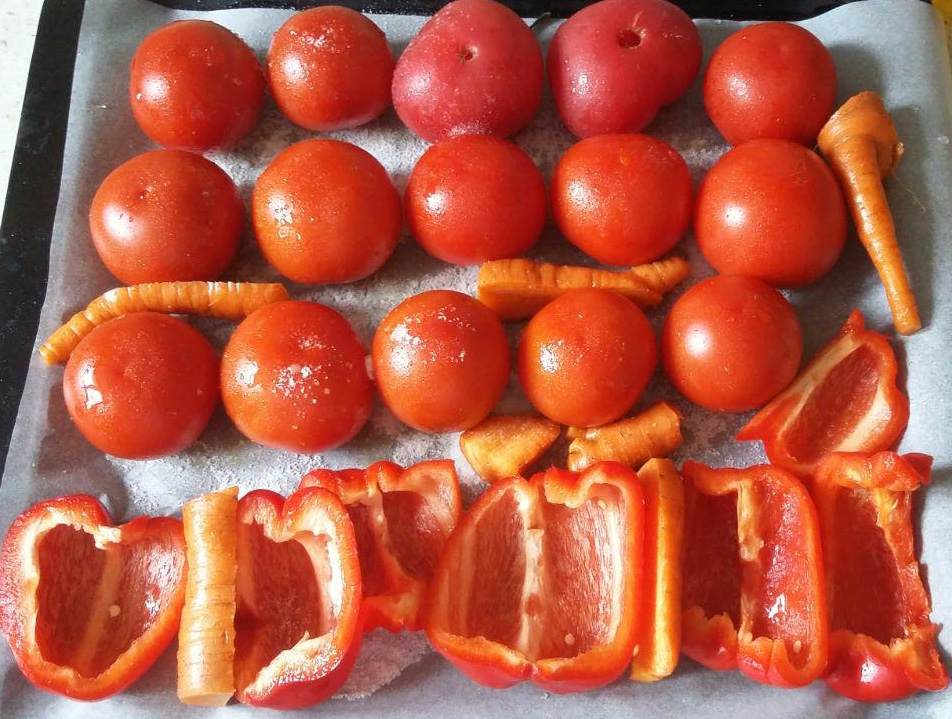
\includegraphics[width=6.5cm]{pic/roasted_peppers}
\end{figure}

\newpage

\section{Desserts}
\begin{recipe}
    [% 
        preparationtime = {\unit[15]{min}},
        portion = {\portion{4}},
        bakingtime = {\unit[25]{min}}
    ]
    {Aquafaba brownie}
    \introduction{%
        Aquafaba is the viscous water from chickpea can. Why should you be bothered? You could possibly exchange it for beaten egg whites but I always struggle what to do with leftover yolks. Aquafaba is a by-product and it's ingenious it can be turned into desserts. Eat chickpea for lunch and aquafaba for afternoon tea - two birds with one stone!
    }

    \ingredients{%
        \unit[200]{g} & Chocolate \\
        \unit[150]{g}  & Butter \\
        1 can & Aquafaba \\
        0.75 c. & Sugar \\
        1.25 c. & Flour \\
        Pinch & Salt \\
        0.25 ts. & Baking powder \\
        & Chili or cinnamon or vanilla \\
        & Raspberries \\
        & Hazelnuts
    }

    \preparation{%
        \step In a small pot heat up gently butter, chocolate and spices till chocolate melts.
        \step Beat aquafaba in an exactly same way as you would do egg whites. At the end add sugar in small portions. Gently mix with melted chocolate.
        \step In a separate bowl, mix flour and baking powder.
        \step Gently, in portions, add flour to liquid and stir with a spatula.
        \step Pour cake batter to a baking tin (small, something like 20x25) lined with parchment. Decorate with nuts, raspberries and pieces of chocolate.
        \step Bake at \unit[180]{\textcelcius} for 20 min. Do not overbake!
    }

    \hint{%
        Add 0.25 cup of coffee to the first step for extra deep flavour.
    }

\end{recipe}
\newpage
\begin{recipe}
    [% 
        preparationtime = {\unit[30]{min}},
        bakingtime = {\unit[30]{min}}
    ]
    {Sweet buns with curd cheese}
    \introduction{%
        Curd cheese is essential. It's high time for a trip to a polish shop. If there's big polish diaspora  in the city, sometimes you can buy it in Tesco but don't confuse it with quark, it's something different (see introduction to a polish shop for details).

        More fancy version involves raspberries or fresh apricots (halfs) and crumble topping
    }

    \ingredients{%
        \unit[500]{g} & Flour \\
        \unit[40]{g}  & Yeast fresh* \\
        2 tbs. & Sugar \\
        2 ts. & Sugar (leaven) \\
        1 c. & Milk \\
        2 & Eggs \\
        50 g. & Melted butter \\
        Filling  &  \\
        400 g & Curd cheese \\
        1 & Egg yolk \\
        0.5 c. & Sugar \\
        \unit[50]{g} & Butter, melted
    }

    \preparation{%
        \step Leaven: dissolve yeast in warm milk (heat milk so you can easily dip your finger in without burning yourself). Add 2 teaspoons of sugar and 1 of flour. Leave in dark cupboard for about 10 min. \underline{Watch out!} It grows, make sure there's enough room in mug/pot/bowl.
        \step Knead dough (start with flour, leaven and eggs, then add melted butter), cover with a cloth and leave in warm place (cupboard, room) for 30-60 min (the dough should almost double its size).
        \step In meantime, blend curd cheese with egg yolk, butter and sugar. It should be smooth and creamy.
        \step Form round, quite flat buns. Leave for 15 min to grow (cover with cloth).
        \step With the help of glass, form a valley in the middle and fill it with cheese. If using raspberries, add them now, on the cheese (press in cheese).
        \step \underline{Bake at \unit[180]{\textcelcius} for 20 min.}
    }

    \suggestion
    {%
        For buns and bread I prefer to use fresh yeasts. Usually I buy them in polish shop. Nevertheless, dried yeast should work too. My converter: 15g fresh ~ 7g dried.

        If you use dried yeast, there's no need to do a leaven (in theory). I usually like to do it anyway.
    }

    \hint{%
        Bone of contention: Magda believes that when doing yeast dough, it shouldn't be in contact with metal surface (spoon, bowl etc) (apart for fork which is necessary to prepare leaven). Hubert doesn't believe in such a thing.
    }

\end{recipe}
\newpage
\begin{recipe}
    [% 
        preparationtime = {\unit[20]{min}},
        bakingtime = {\unit[15]{min}}
    ]
    {Chickpea cookies}

    \introduction{%
        I know that for Bethan 'a treat is a treat' but I believe that there are plenty of puddings and snacks that are not only scrumptious but also carry some nutrients. Incorporating pulses and vegetable to desserts in an endless adventure.
    }

    \ingredients{%
        1 can & Chickpea \\
        0.5 c. & Peanut butter \\
        0.25 c. & Honey \\
        2 heaping tbs. & Flour \\
        50 g & Chocolate, chopped into small pieces \\
        1 ts. & Cinnamon \\
        0.5 ts. & Baking powder }

    \preparation{%
        \step With the help of a blender, mix all ingredients apart for flour and chocolate.

        \step When chickpea is well mashed, add flour and continue blending. Mix chocolate in (use spatula).

        \step Using a spoon form cookies (line baking tray with baking paper) \underline{Bake at \unit[180]{\textcelcius}} \underline{for 15 min till brown.}
    }

\end{recipe}
\newpage
\begin{recipe}
    [% 
        preparationtime = {\unit[5]{min}},
        bakingtime = {\unit[20]{min}}
    ]
    {Rhubarb compote}

    \introduction{%
        When you fancy something nice to drink but don't want to reach for rich in sugar juices - go for compote!
        You can prepare compote from pretty much any seasonal fruit.
        My favourite one is rhubarb compote (M.), then plum and White Transparent apple (not sure if you can get theme here...).
    }

    \ingredients{%
        800 & Rhubarb \\
        2 l & Water \\
        & Sugar \\
        hfl. & Mint \\
        hfl. & Berries
    }

    \preparation{%
        \step Cur rhubarb into 3-4 cm long pieces.
        Fry with a little bit of sugar.

        \step Add 2 l of water and simmer for about 15 min.
        After 10 min, add berries and mint.

        \step Add more sugar if needed.
    }

\end{recipe}
\newpage
\begin{recipe}
    [% 
        preparationtime = {\unit[15]{min}},
        portion = {\portion{4}},
        bakingtime = {\unit[30]{min}}
    ]
    {Rhubarb crumble}

    \introduction{%
        There are three reasons why I love crumbles: preparation is super quick;
        no wheat; little sugar yet is very sweet due to fruit.
    }

    \ingredients{%
        600-800 g & Rhubarb \\
        5 & Apricots \\
        2 hfl. & Berries \\
        2 hfl. & Blueberries (fresh or frozen) \\
        & \\
        100 g. & Butter \\
        \nicefrac{1}{2} c. & Sugar \\
        1~\nicefrac{1}{2} c. & Oat flakes \\
        3 tbs. & Coconut milk powder \\
        1 tbs. & Ginger \\
        \nicefrac{1}{4} ts. & Salt
    }

    \preparation{%
        \step Cut rhubarb into 2-3 cm long pieces, apricots into quarters.
        Mix with berries in an oven dish/tin.


        \step In a hand blender s-shaped knife container (or using your hands) mix all ingredients for crumble topping.
        Add more fat/oats if needed


        \step Cover fruit with crumble topping. \underline{Bake at}
        \underline{\unit[180-200]{\textcelcius} for 20-30 min} till brown.
    }

    \hint{%
        Serve with ice cream or clotted cream.
    }

\end{recipe}


\begin{figure}[h]
    \centering
    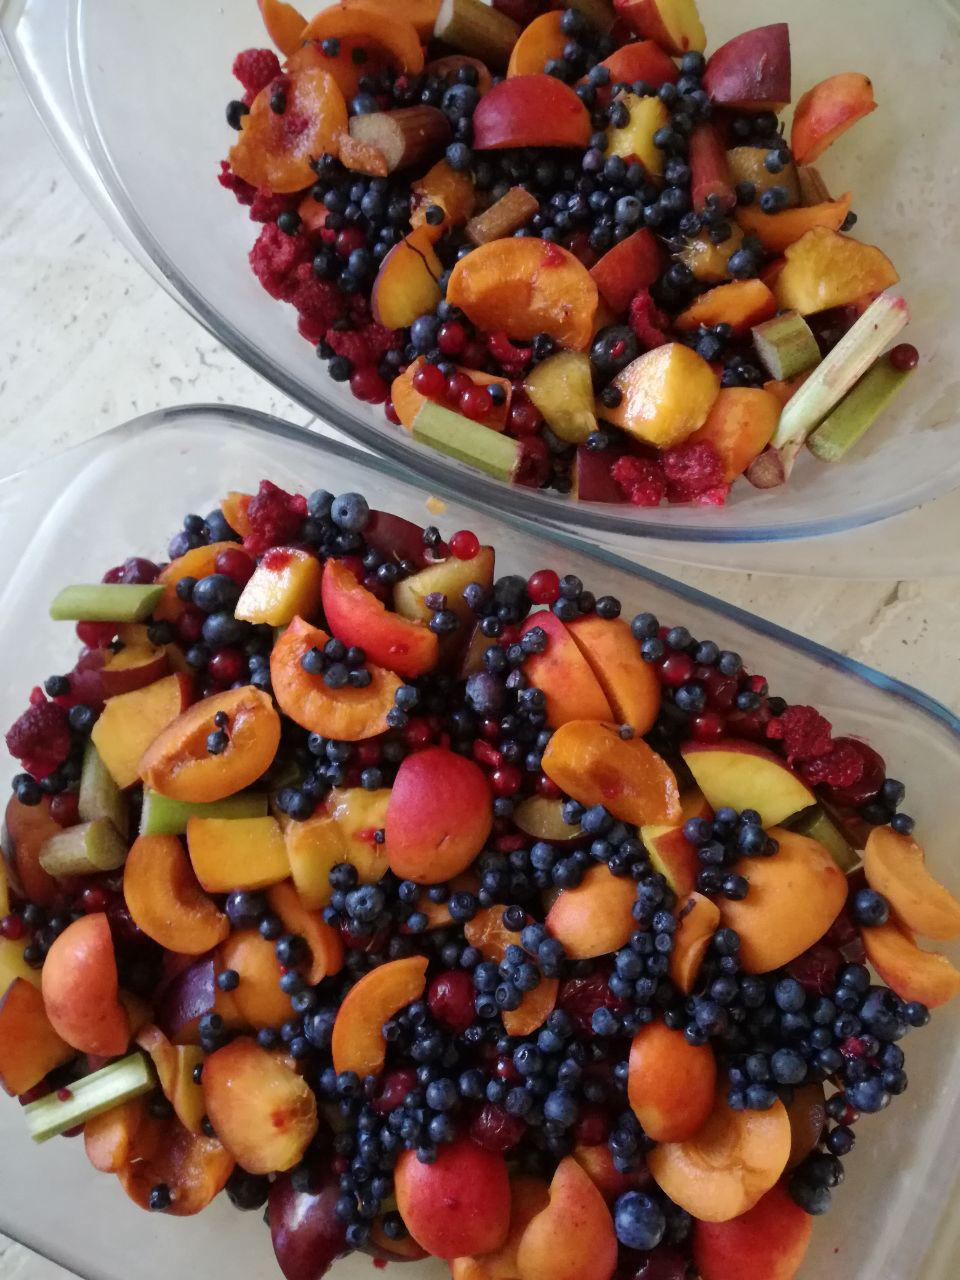
\includegraphics[width=12cm]{pic/crumble}
\end{figure}

\newpage
\begin{recipe}
    [% 
        preparationtime = {\unit[25]{min}},
        bakingtime = {\unit[45]{min}},
        portion = {one good party},
        source = {kwestiasmaku.com: lesny-mech}
    ]
    {The forest moss cake}

    \introduction{%
        Fear not, you won't be able to sense the taste of the spinach (partly because it doesn't have much taste anyway); I've tested that on my family.
    }

    \ingredients{%
        & pomegranate \textbf{and/or} \\
        & blueberries \\
        & fresh basil \\
        & \textbf{Cake} \\
        \unit[450]{g} & spinach \\
        \unit[1/2]{c.} & oil \\
        \unit[1/2]{c.} & sugar \\
        3 & eggs \\
        \unit[2]{c.} & flour \\
        \unit[2]{tsp} & baking powder \\
        & \textbf{Cream} \\
        \unit[250]{g} & mascarpone \\
        \unit[200]{ml} & crème fraîche \\
        % TODO: verify this is appropriate for 30% sour cream
        & icing sugar \\
        \unit[1]{tsp} & vanila extract \\
        & polymer to hold the cream
        % TODO: śmietanfix
    }

    \preparation{%
        \step Defrost spinach if needed, blend into a uniform paste.
        If you have fresh spinach, heat it up for 3 minutes on a pan first.

        \step Preheat the oven to \unit[180]{\textcelcius}. Crack the eggs into a bowl, add sugar and beat.
        Continue beating while slowly pouring in the oil.
        Add the spinach and blend (low power) until the two ingredients mix.

        \step Mix the flour with baking powder, add to the mixture and briefly blend again.
        Pour the mix into a round form and bake for \unit[40-45]{minutes} until dry inside.
        Take out and cool down to room temperature.

        \step Beat all the cream ingredients until stiff.
        % TODO: add śmietan-fix

        \step Cut off the top third of the cake.
        Spread the cream on the bottom part.
        Break the top into small crumbs and use them to decorate the cream.
        Decorate with fruit and basil leafs.
    }

    \hint{%
        Reportedly beating the eggs is easier if they are warm.
        Put them into hot tap water for 10 minutes.
    }

\end{recipe}

\newpage

\begin{recipe}
[% 
    preparationtime = {\unit[0.5]{h}},
    bakingtime={\unit[1]{h}},
    bakingtemperature={\protect\bakingtemperature{
       topbottomheat=\unit[195]{dC}},
    portion = {\portion{6-8}},
    source = {polish wisdom}
]
{Strawberry cake}
    
    
    \introduction{%
        \blindtext
    }
    
    \ingredients{%
        \textbf{Sponge}  & 
        5  & eggs\\
        \unit[3/4]{c} & Sugar\\
        \unit[3/4]{c} & Flour\\
        \unit[1/4]{c} & Starch (Potato or corn)\\
        \textbf{Cream} & 
        \unit[3]{c} & Milk\\
        \unit[3/4]{c} & Sugar\\
        \unit[4]{tbs} & Flour (heaped spoonful )\\
        \unit[4]{tbs} & Starch (heaped spoonful)\\
        \unit[150-250]{g} & Butter\\
        1 & Egg yolk\\
    }
    
    \preparation{%
        \step All ingredients for sponge must be at room temperature. Beat whites until stiff. While still beating, add sugar (one spoon at the time). Then egg yolks (one at the time, still beating gently).   
        \step Add sifted flour. \underline{Don't beat.} Gently mix with a spatula.
        \step Line the cake tin with parchment (only bottom), don't grease sides. Fill with batter. Bake at 160-170$^\circle$C for 35-40min. 
        \step Boil 2/3 milk and sugar up. In a cup or high blender dish mix (with fork or a beater) flour, yolk and remaining milk. When sugar/milk liquid is boiling, add flour/milk and stir vigorously for about 2 min. Remove from heating and continue stirring. 
        \step Cool the blancmange (step 4). Cream butter and mix with blancmange (add in small portions).
        \step Sandwich the sponge and decorate with fresh fruit!  
    }
    
    \suggestion[Spice it up!]
    {%
      To make chocolate cream, add cocoa powder to milk-flour mixture. 
    }
    
   
    
    \tipp{%
        Drop hot sponge in the tin on the kitchen bench/floor from 30cm. Trust me, it will keep the cake fluffier.
    }
    
\end{recipe}
\newpage
\begin{recipe}
    [% 
        preparationtime = {\unit[30]{min}},
        bakingtime = {\unit[60]{min}}
    ]
    {Tofu pumpkin 'cheesecake'}
    \introduction{%
        This recipe it's quite time-consuming.
        You have to cook millet, prepare pumpkin purée and gather all the ingredients.
        The cake is, however, spectacular, so let's celebrate!

        Coconut milk must be from the can as this one is rich in fat that adds mellowness to the cake.

        Millet makes the cake more dense and less spongy.

        Lemon juice is essential to turn tofu into more 'cheesy' base.

        Long blending is essential for creamy texture!
    }

    \ingredients{%
        \unit[150]{g} & Digestives \\
        3 tbs. & Peanut butter \\
        Pinch & Salt \\
        & \\
        \unit[360]{g} & Natural tofu \\
        0.5 c. & Pumpkin purée \\
        0.75 c. & Cooked millet \\
        0.75 c. & Caster sugar \\
        2 tbs. & Starch \\
        1 ts. & Cinnamon \\
        1 ts. & Cardamom \\
        1 ts. & Ginger \\
        0.25 ts. & Nutmeg \\
        &  \\
        1 c. & Coconut milk (from the can) \\
        0.25 c. & Orange juice \\
        0.25 c. & Lemon juice \\
        & \\
        75 g & Dark chocolate \\
        0.5 c. & Coconut milk (can)*
    }

    \preparation{%
        \step \textbf{Base}: blend negligently.
        Press into lined with parchment cake tin.
        Refrigerate.
        \step \textbf{Cake}: Blend thoroughly everything apart from: milk, lemon and orange juice.
        When dough is smooth, gradually add liquids.
        \step Pour onto the base.
        Bake at\underline{ \unit[180]{\textcelcius}} for 15 min.
        \step Then, turn the oven down to  \underline{\unit[120]{\textcelcius}} and bake for about 45 min.
        Switch the oven off but \underline{leave the cake in} for another 15 min.
        Cool down for 2h.
        \step \textbf{Coating}: Heat all ingredients in a small pot, till chocolate melts.
        Leave for 20 min to cool down, pour over \underline{cold} cake.
        \vspace{35mm}
    }
    \suggestion
    {%
        *For chocolate coating, you can use single cream instead but reduce the amount to about 1/3 cup.
        For sweeter coating, add caster sugar.
    }

    \hint{%
        When you turn temperature down to 120, you can add oven dish full of close to boiling temperature water at the bottom of the oven.
        Steam will stop the cake from cracking.
    }

\end{recipe}
\newpage

\section{Dinner}

\begin{recipe}
    [% 
        preparationtime = {\unit[0.5]{h}},
        portion = {\portion{3-4}},
        bakingtime = {\unit[0.5]{h}}
    ]
    {Tart with beetroot and goat cheese}
    
    \introduction{%
        This tart is sooo easy to do.
        And quite spectacular.
        Add salad, wine, candles... more wine ;)
    }

    \ingredients{%
        & Puff pastry \\
        3 & Cooked/baked beetroot \\
        \unit[200]{g} & Goat cheese \\
        4 & Eggs \\
        \unit[200]{ml} & Sour cream \\
        1 tbs. & Flour \\
        & Thyme \\
        & Balsamic vinegar
    }

    \preparation{%
        \step Mix eggs, cream, flour and spices.

        \step Slice beetroot and goat cheese.

        \step Line oven dish with puff pastry, make a few holes with a fork.
        Blind bake for 5 min.

        \step Layer beetroot, then cheese.
        Pour over egg mixture. \underline{Bake for 25-30 min at \unit[180]{\textcelcius}.}

        \step  Sprinkle with balsamic vinegar.
    }

\end{recipe}

\begin{figure}[h]
    \centering
    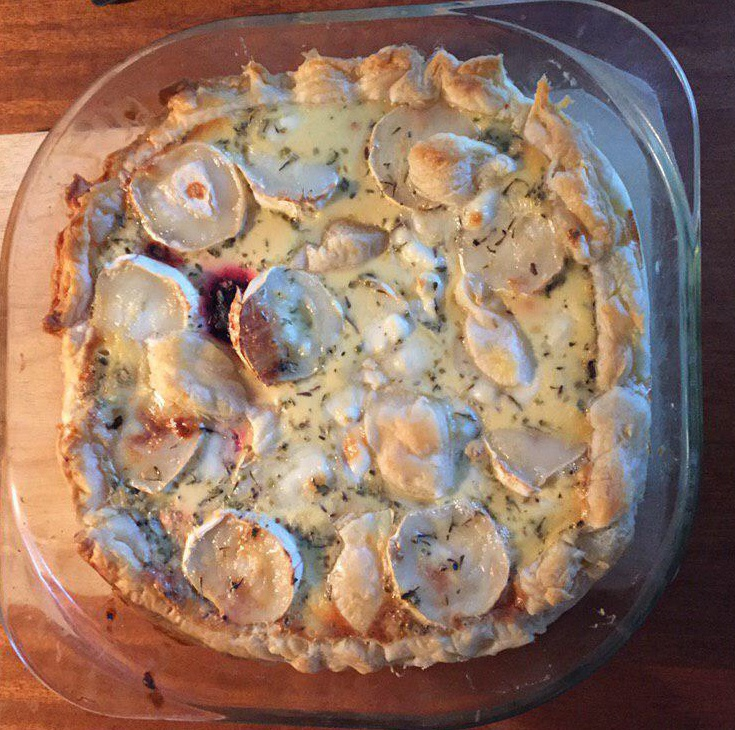
\includegraphics[height=9cm]{pic/beetroot_cheese}
\end{figure}

\newpage
% Complete recipe example
\begin{recipe}
[% 
    preparationtime = {\unit[0.5]{h}},
    portion = {\portion{3-4}},
    bakingtime={\unit[0.5]{h}}
]
{Carrot \textit{kopytka}}
    
    
  
    \ingredients{%
    	\unit[500]{g} 	& Carrot purée \\
    	\unit[200]{g} 	& Starch \\
    	\unit[200]{g} 	& Corn flour \\
    	2 tbs. & Yeast flakes \\
        & Nutmeg \\
       
        \textbf{Sauce} & 
        5 & Garlic cloves \\
        2 tbs. & Tahini \\
        2 tbs. & Soy sauce \\
        1/2 & Lime\\
        2 tbs. & Sesame oil \\
        1 ts. & Coriander \\
        1 ts. & Cumin \\
        
     
    }
    
    \preparation{%
        \step  Boil 5l of water.
        \step Knead all ingredients for dough. Roll and cut into small rods (see picture). 
        \step Cook \textit{kopytka} in hot water till tender (about 3 min from the moment when they started floating - as opposed to stay at the bottom of the pot).
        \step Heat frying pan with some oil. Add all ingredients of the sauce (do it in chunks if you're not going to fit all of the \textit{kopytka} at once).
        \step  Fry \textit{kopytka} and covered in sauce. Serve with greens. 
       
    }
    
 
    
    
\end{recipe}
\newpage
% Complete recipe example
\begin{recipe}
[% 
    preparationtime = {\unit[15]{h}},
    portion = {\portion{4}},
    bakingtime={\unit[25]{min}}
]
{Chicken breasts in curry coconut milk}

    
  
    \ingredients{%
    	2 & Chicken breast \\
       2 can & Coconut milk\\
       & Tumeric \\
        & Curry powder\\
       	& Paprica \\
      	& Coriander  \\
       	& Cumin \\
        & Garam masala 
     }
    
    \preparation{%
        \step Cut each breast into 4 elongated pieces. 
        \step Toss meat in spices (+salt), line in the oven dish and cover with coconut milk.
        \step Bake for 20-25 min at \unit[180]{\textcelcius}).
        }
    
  \hint{%
 	Serve with rice (add lemon juice and coriander leaves) and green beans and peppers fried with garlic and a hint of soy sauce}
    
\end{recipe}
\newpage
\begin{recipe}
    [% 
        preparationtime = {\unit[30]{min}},
        bakingtime = {\unit[1]{h}},
        portion = {\portion{4}}
    ]
    {Curry with sweet potatoes and butternut squash}

    \setRecipeLengths{
        ingredientswidth=6cm
    }
    \ingredients[15]{%
        1 & Onion \\
        1 & Sweet potato \\
        1 & Butternut squash \\
        2 can & Tomatoes \\
        \unit[2]{c.} & Kale \\
        1-2 cans & Chickpea \\
        1 can & Coconut milk \\
        & \\
        & Curry powder \\
        & Turmeric \\
        & Coriander \\
        & Cumin \\
        & Garam Masala \\
        & Cinnamon \\
        & Cloves
    }

    \preparation{%
        \step Dice onion, chop up sweet potato and butternut squash.

        \step  Fry onion with spices.
        Add canned tomatoes and veg apart from kale.
        Simmer for about an hour.

        \step Add kale, chickpea and coconut milk, keep heating for 5 min.
    }


    \hint{%
        Butternut squash can be swapped for carrots, kale for spinach and chickpea for other pulses.
    }
\end{recipe}

\begin{figure}[h]
    \centering
    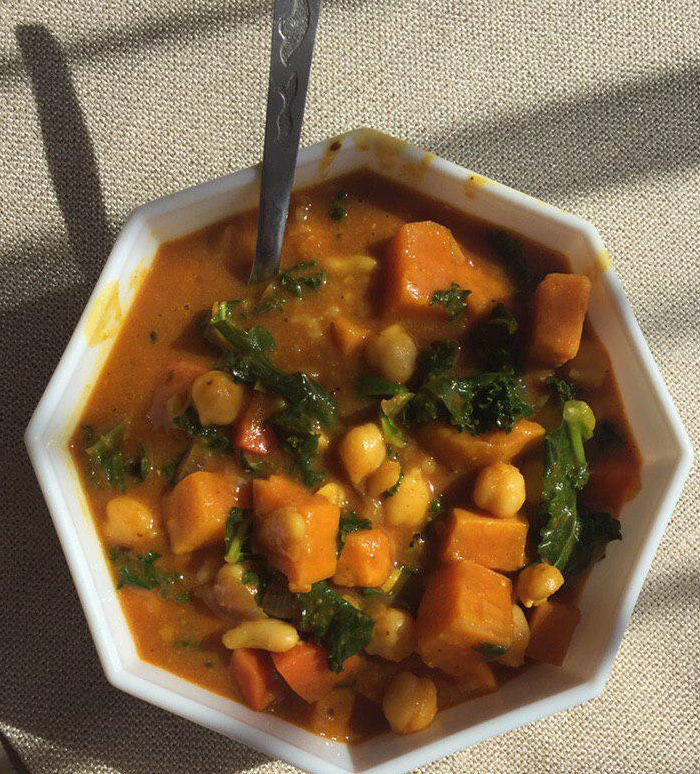
\includegraphics[width=12cm]{pic/curry_sweet_potato}
\end{figure}

\newpage
% Complete recipe example
\begin{recipe}
[% 
    preparationtime = {\unit[1]{h}},
    portion = {\portion{2}},
    bakingtime={\unit[40]{min}}
]
{Roast pepper and cheese galette}
    
    \introduction{%
    	Whenever I think about fancy dinner (supper?), I reach for stuffed pastry. Ladies and gentlemen, tonight we're serving French galette!
    }
    
  
    \ingredients{%
    	\unit[200]{g} & Flour \\
       1/4 tbs. & Salt\\
       \unit[100]{g} 	& Butter \\
        \unit[100]{g}  & Sour cream \\
       \textbf{Filling }&  \\
       2 & Pepper \\
       1 & Garlic clove \\
       \unit[100]{g} 	& Ricotta \\
       \unit[50]{g} 	& Cheese (eg. Grana Padano) \\
       \unit[50]{g} 	& Mozzarella \\
        & Fresh basil
     }
    
    \preparation{%
        \step Mix flour, salt and cold butter. Add sour cream and quickly knead the dough. If needed, add spoon or two of cold water. \underline{Cover with foil and leave in the fridge for an hour.}
        \step Roast slices of pepper (30 min, \unit[200]{\textcelcius})
        \step In a bowl, mix garlic and olive oil, salt and pepper to taste.
        \step On bench covered with flour, stretch the dough to form a circle, place it on parchment. In the middle (leaving about 5 cm edge) spread ricotta, mozzarella and Grana Padano. Place pepper on the cheese, starting with the outer edge of the cheesy filling.  
        \step  Wrap free edges towards the centre (see picture).
        \step Bake for 30-40 min.
        \step Garnish with basil leaves. 
       
    }
    
  \hint{%
 	If the dough is very gluey, wet your hands for easier handling. }
    
\end{recipe}
\newpage
\begin{recipe}
    [% 
        preparationtime = {\unit[1.5]{h}},
        portion = {\portion{4}},
        bakingtime = {\unit[0.5]{min}}
    ]
    {Polish croquette with spinach and feta cheese}

    \ingredients[20]{%
        2 c. & Flour \\
        4 & Eggs \\
        2 c. & Milk \\
        1.5 c. & Water \\
        pinch & Salt \\
        2 tbs. & Oil \\
        & \\
        800 g & Spinach \\
        5 & Garlic cloves \\
        200 g & Feta cheese \\
        & Nutmeg \\
        & \\
        & Breadcrumbs \\
        & Beaten egg
    }

    \preparation{%
        \step Mix all ingredients for crepes batter. Fry crepes on a greased frying pan.

        \step Fry spinach, nutmeg and garlic till most of the water from spinach evaporates. Then add crushed feta cheese and mix well.

        \step Croquette folding - see picture.

        \begin{figure}[!h]
            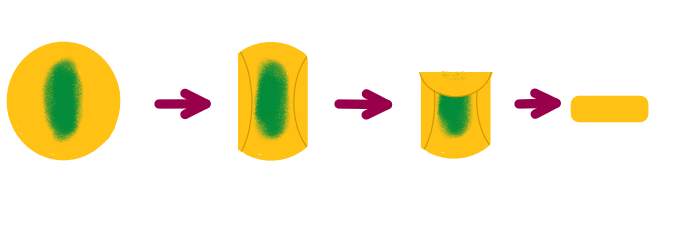
\includegraphics[width=.6\linewidth]{krokiety}
        \end{figure}

        \step Folded croquettes dip in beaten egg (with salt and pepper) and then cover with breadcrumbs. Fry till brown (you'll need relatively lots of oil).
    }

    \suggestion{%
        Now try different fillings. Maybe mushroom, pepper and cheddar?
    }

\end{recipe}
\newpage
% Complete recipe example
\begin{recipe}
[% 
    preparationtime = {\unit[1]{h}},
    bakingtime={\unit[1]{h}},
    portion = {\portion{4-5}}
]
{Lasagne with pumpkin and millet}
    
    \ingredients{%
        \unit[2]{c} & Pumpkin purée \\
        \unit[3/4]{c} & Millet \\
        \unit[200]{ml} & Cream \\
        Handful & Capers \\
        Handful & Dried tomatoes \\
        & Sage \\
        Box	& Lasagne sheets \\
        \textbf{Sauce} & \\
        2 cans & Tomatoes \\
        \unit[400]{ml} & Passata \\
        1 & Onion \\
        & Smoked paprika \\
        & Balsamic vinegar \\
        & \\
        & Cheese for topping - mozzarella or grated cheddar
    }
    
    \preparation{%
        \step Rinse millet with boiling water. Add 1.5 c of water, salt and cook at small heat till millet absorbed all liquid. If still not tender, add more water and cook till tender. When cooking millet, leave it alone, don't stir it, don't uncover it etc. 
        \step Fry onion, add all sauce ingredients and simmer for as long as you can.
        \step Mix with blender cooked millet, pumpkin purée and remaining filling ingredients apart for capers and dried tomatoes. Add capers and chopped dried tomatoes.  
        \step In high oven dish layer alternately sauce, lasagne sheets, pumpkin filling and lasagne sheet. End with sauce, add cheese on the top.
        \step Bake for about an 1h (check if pasta is tender).
    }
    
    \suggestion[]
    {%
       You can also prepare béchamel sauce and either alternate it with tomato sauce or replace. 
    }
    
    
    \hint{%
        For extra umami flavour, add yeast flakes to the pumpkin filling or cook millet in broth. 
    }
    
\end{recipe}
\newpage

\begin{recipe}
[% 
    preparationtime = {\unit[0.5]{h}},
    bakingtime={\unit[30]{min}}
]
{Best wege patty; Polish edition}
    
    \ingredients{%
        2 c. & Grated carrot \\
        0.75 c. & Millet \\
        0.5 c.  & Roast sunflower seed \\
        0.5 c. & Roast sesame \\
        1 & Red onion \\
        0.5 c. & Breadcrumbs \\
        0.25 c. & Oil \\
        3 tbs. & Flour \\
        4 tbs. & Soy sauce \\
        2 ts. & Coriander powder \\
        0.5 bunch & Parsley \\
        1 ts. & Ginger \\
        & Chili \\
        &Sat\&pepper 
    }
    
    \preparation{%
        \step Cook millet: rinse with water, rinse well with boiling water, cook in 2.25 c. of hot salted water, covered, for 12-15 min. Don't stir.
        \step Dice onion and chop parsley. Mix all ingredients. 
        \step If the mixture is not gluey enough, add more oil/flour.
        \step Form patties and put on baking paper.
        \step Bake at \unit[200]{\textcelcius} for 30 min, turn patties after 15 min.
    }
    
    \suggestion
    {%
      Serve either as burgers, in buns, or as main dish with roast vegetables. Mango chutney, good (why not home-made?) ketchup or garlic dip go well with patties.
    }
\hint{%
	Watch out, it's very easy to burn sesame when roasting!
}
    
\end{recipe}
\newpage
\begin{recipe}
[% 
    preparationtime = {\unit[15]{min}},
    bakingtime={\unit[20]{min}},
    portion = {\portion{3-4}},
    source = {My Headmaster \& Giovanni Burro}
]
{Pizza dough}

    \ingredients[8]{%
        \unit[150]{g} & wholemeal flour \\
        \unit[350]{g} & white flour \\
        \unit[25]{g} & fresh yeast \\
        \textbf{or} & \\
        \unit[7]{g} & dried yeast \\
        \unit[250]{ml} & milk \\
        \unit[2]{Tsp} & olive oil \\
        \unit[1]{tsp} & salt \\
        \unit[1]{tsp} & sugar
    }
    
    \preparation{%
        \step Warm up the milk to about \unit[40-50]{\textcelcius} and dissolve the yeast with sugar (hot water may kill the yeast!). Leave them to 'wake up' for \unit[5-10]{minutes}. You need a larger glass to accommodate some foam.
        
        \step Mix together the two types of flour, salt and oil. I prefer to start in a bowl, stirring with a table spoon. 
        
        \step Gradually add the milk, stirring constantly. The dough should be sticky but not wet: balance with extra flour or warm water as needed.
        
        \step Put the dough on a flat, clean (Bethan, I'm watching you!)
        % TODO: sanitize
        surface and pug for 5 minutes. The goal is to create bubbles of air inside so you should push the dough with the bottom of your palm(s) and them fold in half. 
        \step Leave it to grow for at least 20 minutes in a warm place, covered with a cloth. Roll to \unit[3-5]{mm} thickness and bake for about 20 minutes at \unit[185]{\textcelcius} with your favourite toppings. 
    }
    
    \hint{%
        Equation for yeast growth is exactly the same as for bacteria growth: moderate temperature, moisture, food, oxygen and time. That's why the later like washing-up sponges so much...
    }

\end{recipe}
\newpage
\begin{recipe}
    [% 
        preparationtime = {\unit[30]{min}},
        portion = {\portion{4}},
        bakingtime={\unit[25]{min}}
    ]
    {Courgette 'potato pancakes'}
    \introduction{%
        First and foremost, it has nothing to do with a sweet crepes you would serve for breakfast. It's a savoury dish, traditionally made of potatoes, onion and flour; served with sour cream and salt or sugar (apparently half of Poland eats it with sugar, personally, I beg to differ...).

        What I present to you here is an upgraded version. Potatoes out, courgette in.

        You can serve with simply with sour cream or garlic dip, chilli sauce, chutney...
    }

    \ingredients{%
        \unit[600]{g} & Courgette \\
        1 & Onion \\
        Half bunch & Parsley \\
        Half bunch & Dill \\
        100 g & Feta cheese \\
        0.5 c. & Yoghurt \\
        2 & Egg \\
        \unit[100]{g} & Flour \\
        & Nutmeg \\
        & Salt\&pepper
    }

    \preparation{%
        \step Grate courgettes, salt. Leave for 15 min. Then drain well.
        \step Mix eggs, yoghurt, onion, herbs and spices. Add flour. Then grated courgette.Texture should be similar to dense pancake batter.
        \step Fry on preheated oil till brown (form pancakes with spoon or small ladle).
    }

    \hint{%
        This is only an introduction... Why not to try sweet pumpkin version with quark and ginger? Or grated celeriac, oats and parsley?
    }

\end{recipe}
\newpage
\begin{recipe}
	[% 
		preparationtime = {\unit[20]{min}},
		portion = {\portion{4}},
		bakingtime = {\unit[35]{min}}
	]
	{Favourite tomato pasta sauce}
	\introduction{%
		The tastiest version is if you use: tagliatelle pasta and dried mushrooms.
        I use 'continental' mushrooms, not Asian, so something like: bolete or porcini.

		If you can't buy celeriac, use more parsnips instead.
	}

	\ingredients{%
		\unit[300]{g} & Pasta, raw \\
		1 & Celeriac \\
		2-3 & Carrot \\
		1 & Parsnip \\
		Handf. & Dried mushrooms \\
		\unit[1]{l} & Passata \\
		0.5 c. & Red lentil \\
		2 & Onion \\
		5 & Allspice \\
		5 & Bay leaves \\
		3 tbs. & Soy sauce \\
		1 ts. & Coriander \\
		1 ts. & Cumin \\
		1.5 ts. & Smoked paprika \\
		2 tbs. & Balsamic vinegar \\
		& Hot paprika/chilli
	}

	\preparation{%
		\step Dice carrots, parsnip, celeriac and onion.
        Fry with bay leaves, chopped dried mushrooms and allspice for about 10 min.
		\step Add lentil, glass of water (add more later if necessary) and half of the passata + spices and vinegar, simmer for 10 min.
		\step Add more passata and simmer for another 15min, add more liquid if necessary (passata/water).
	}

	\hint{%
		The longer the simmering, the richer the flavour!
	}

\end{recipe}
\newpage
\begin{recipe}
    [% 
        preparationtime = {\unit[1]{h}},
        portion = {\portion{3-5}},
        source = {Magda's first cookbook}
    ]
    {Pork loin with baby carrots}

    \setRecipeLengths{
        ingredientswidth=5.5cm
    }

    \ingredients[17]{%
        \unit[200]{g} & bulgur or millet \\
        & \textbf{Carrots} \\
        \unit[500]{g} & baby carrots \\
        \unit[50]{g} & butter \\
        \unit[2]{Tsp} & honey \\
        a bit & chilli powder \\
        a lot & cinnamon \\
        & powdered ginger \\
        & \textbf{Pork} \\
        \unit[500]{g} & pork loin \\
        3-5 claws & garlic \\
        & flour \\
        & paprika \\
        & smoked paprika \\
        & soy sauce \\
        & herb pepper \\
        & salt \& pepper
    }

    \preparation{%
        \step Melt the butter and fry the carrots for 5 minutes, stirring.
        They should cover the whole pan.
        Pour boiling water to cover the carrots, put a lid on.

        \step when the carrots get soft-ish, add honey and spices, stir.
        Evaporate the water and let the honey caramelise.

        \step Boil the millet in salted water or vegetable stock.
        Stir in some butter if it is ready too early.

        \step Cut the pork loin into \unit[10-15]{mm} wide slices.
        You may smash it a bit.
        % TODO: vocab smash

        \step Mix all remaining spices (except for garlic) with a small amount of flour.
        The soy sauce should make the seasoning sticky but not watery.
        Cover the meat with all the seasoning.

        \step preheat a pan with a fair amount of oil (strong heat).
        Fry both sides of the pork.
        Add whole garlic claws to the pan to reduce oil sparkling.
        Replace them if burned.
        % TODO: vocab strong heat

        \step Pour in some boiling water and let it simmer until the meat is soft.
        Evaporate the water and serve in its own juice.
    }

\end{recipe}
\newpage
\begin{recipe}
    [% 
        preparationtime = {\unit[40]{min}},
        portion = {\portion{4}},
        bakingtime = {\unit[60]{min}}
    ]
    {Stuffed aubergines}

    \introduction{%
        Another meaty recipe. It's quite time-consuming but don't be put off, as the preparation is rather easy.
    }

    \ingredients{%
        2 & Aubergine, big \\
        \unit[500]{g} & Minced beef \\
        \unit[500]{ml} 	& Passata \\
        1 & Onion \\
        4 & Garlic clove \\
        & Mozzarella \\
        3 handf. & Olives \\
        \unit[100]{g} 	& Grated cheddar or Grana Padano  \\
        & Thyme \\
        & Oregano \\
        & Paprika \\
        & Balsamic vinegar
    }

    \preparation{%
        \step Cut aubergines in half. Nick across (care not to cut the skin). Sprinkle with salt and olive oil, bake at \unit[180]{\textcelcius} for 25-30 min.
        \step Fry onion, at the end add garlic. Add mince and fry for 5-7 min.
        \step Core aubergines and chopped flesh add to meat.
        \step Stuff aubergine boats with meat and cover with cheese. Beak at  \unit[160-180]{\textcelcius} for about 10 min.
    }

\end{recipe}
\newpage
\begin{recipe}
    [% 
        preparationtime = {\unit[30]{min}},
        portion = {\portion{2}},
        bakingtime = {\unit[25]{min}}
    ]
    {Trout on vegetables slices}
    \introduction{%
        I think that a well seasoned fresh fish is the most festive dish.
        Add sliced vegetables and pesto to make it more special.
    }

    \ingredients[17]{%
        2 & fresh trout \\
        \unit[2]{tbs.} & Butter \\
        4 & Lemon slices \\
        & Coriander powder \\
        3 & Squeezed garlic cloves \\
        4 & Potatoes \\
        2 & Beetroot (raw!) \\
        & Thyme \\
        4 hfl. & Green leaves* \\
        2 tbs. & Yeast flakes \\
        4 & Garlic cloves \\
        \nicefrac{1}{4} c. & Roast pumpkin seeds \\
        4 tbs. & Olive oil \\
        & Lemon juice
    }

    \preparation{%
        \step Slice (very finely) peeled beetroot and potatoes.
        Blanch potatoes for 5-7 min.
        
        \step In a mortar, grind: coriander, salt, pepper and garlic.
        Add butter and mix.
        
        \step Wash trout and stuff with mixture from the mortar; add lemon slices.
        
        \step Line a tray with aluminium foil, leaving free foil to cover trout later on.
        Layer potatoes (sprinkle with olive oil and thyme) and beetroot.
        
        \step Place trout on vegetables, cover tightly with foil. \underline{Bake at \unit[180]{\textcelcius} for 20-25 min.}
        
        \step \textbf{Pesto:} Blend leaves, garlic, seeds, oil, yeast flake, lemon juice and salt.
        
        \step Serve trout as follows: on the plate layer vegetables, in the middle spread pesto, place rout on the pesto.
    }

    \hint{%
        *Green leaves: in Poland I would normally use either radish leaves or kohlrabi or mixture of both.
        However, I'm aware that if you don't have an allotment you may not be able to buy them in the UK.
        Good alternative will be fresh parsley or carrot top.
    }

\end{recipe}

\begin{figure}[h]
    \centering
    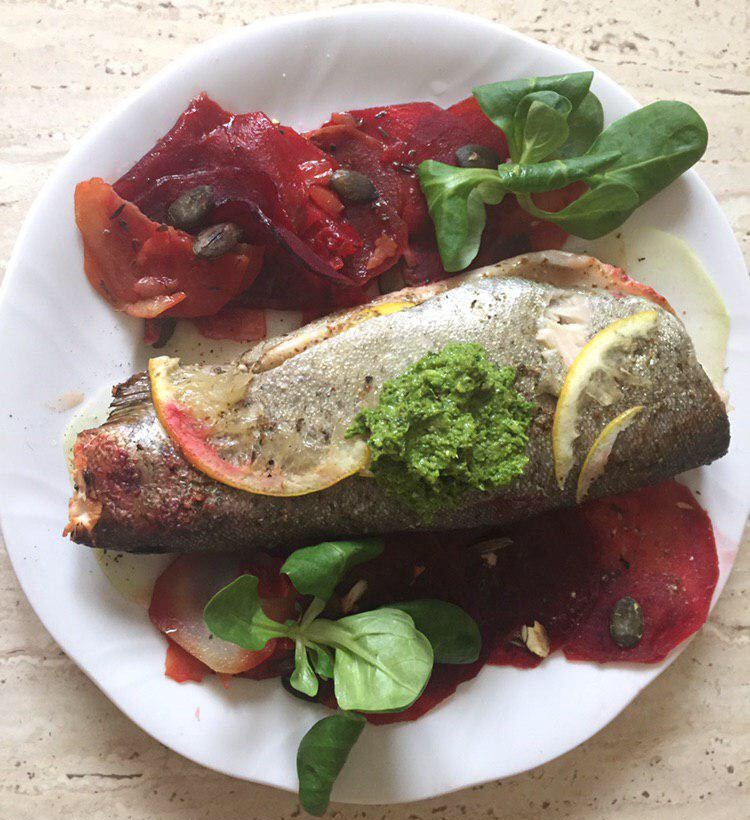
\includegraphics[height=11cm]{pic/trout}
\end{figure}
\begin{figure}[h]
    \centering
    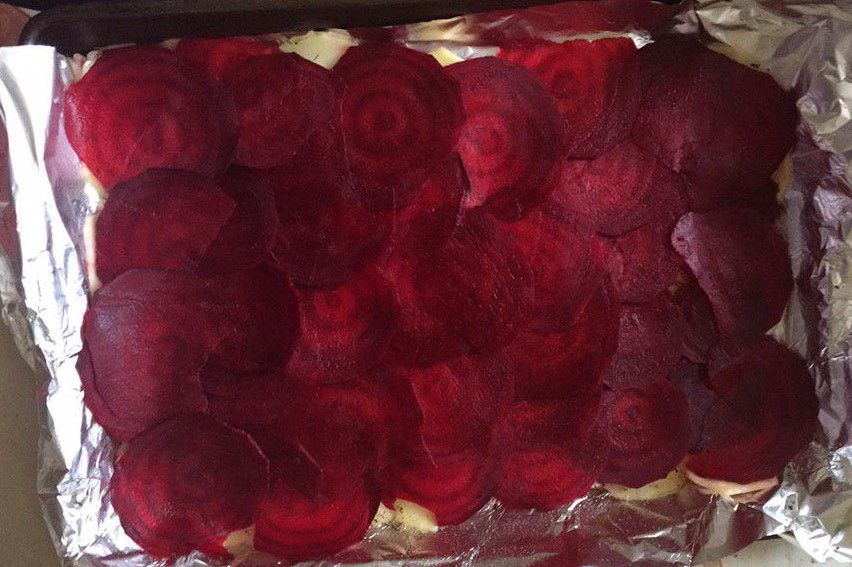
\includegraphics[height=8cm,angle=0]{pic/beetroot}
\end{figure}
% TODO: put images side to side

\newpage

\section{Party/picnic}

% Complete recipe example
\begin{recipe}
[% 
    preparationtime = {\unit[0.5]{h}},
    portion = {\portion{3-4}},
    bakingtime={\unit[40]{min}}
]
{Asparagus tart}

    \ingredients{%
        \unit [200]{g} & Flour \\
        \unit [120]{g} &Butter \\
        1 & Egg \\
        1 ts. & salt \\
        & \\
        Bunch & Asparagus \\
        \unit [200]{ml} & Sour cream \\
        2 & Egg \\
        1 tbs. & Flour \\
        & Nutmeg \\
        & Salt\&pepper \\
        & Thyme
    		}

    \preparation{%
       \step Knead shortcrust pastry. Cover with cling film and refrigerate for 30min. 
       \step Remove lignified ends of asparagus. Wash and cook for 4 min (water shall not cover heads).
       \step Beat eggs, mix with sour cream, flour and spices.
       \step Grease baking dish with butter, line with pastry (roll circle bigger than the dish and transport it on roller). Lay asparagus and pour the egg mix over.
       \step Bake at for about 40 min at \unit[160-170]{\textcelcius}.
             
    }

\end{recipe}
\newpage

\begin{recipe}
    [% 
        preparationtime = {\unit[0.5]{h}},
        bakingtime={\unit[1.5]{h}}
    ]
    {Beetroot carpaccio}

    \introduction{%
        Easy salad, perfect for hot summer garden party or as a starter before fancy dinner.
    }

    \ingredients{%
        4  & Beetroot (elongated ones are the best)\\
        & Feta cheese/goat cheese \\
        & Balsamic vinegar \\
        & Olive oil \\
        & Rocket \\
        & Pumpkin seed/pistachio
    }

    \preparation{%
        \step Cover washed raw beetroot in aluminium foil. Bake till tender (around 1-1.5h)
        \step Slices thinly. Sprinkle with olive oil, black pepper and balsamic vinegar.
        \step Scatter cheese, rocket and seeds. Add extra olive oil and balsamic vinegar.
    }

    \suggestion[Be efficient]
    {%
        It's a lot of faff to bake just a few beetroot. Instead, bake them when baking something different, as they're covered in foil, fragrances shouldn't permeate.
    }

\end{recipe}
\newpage

\begin{recipe}
    [% 
        preparationtime = {\unit[40]{minutes} +  \unit[2]{h} waiting},
        bakingtime = {\unit[30]{min}},
        portion = {40-50 pasties}
    ]
    {Lentil pasties}

    \introduction{%
        These make a marvelous lunch, especially when you go for a whole day trip.
        As meat-free you can store them in a warm backpack without fear...

        The pastry is universal and versatile - you will always succeed.
        The tricky bit is the stuffing - you need to make sure it stands out.
        Nutmeg is your friend here, go for a lot.
        Also, make sure it is rich with umami taste: mushrooms, dried tomatoes, soy sauce are all good sources of it.

    }

    \setRecipeLengths{
        ingredientswidth=5cm
    }
    \ingredients[20]{%
        & \textbf{Pastry} \\
        1 c. & milk \\
        3 c.es & flour \\
        & dried yiest \\
        2 tsp & (cane) sugar \\
        1/2 tsp & salt \\
        1/3 c. & oil \\
        & \textbf{Stuffing} \\
        1 c. & green (brown) lentil \\
        & dried mushrooms \\
        1 & large onion \\
        2 & bay leafs \\
        2 & allspice grain \\
        2 & cloves \\
        & juniper \\
        % TODO: http://www.jadlonomia.com/przepisy/paszteciki-z-soczewica-2/
        5 Tsp & oil \\
        2 Tsp & soy sauce \\
        2 Tsp & milk \\
        & nutmeg \\
        & salt \& pepper
    }

    \preparation{%
        \step Warm up the milk a little bit.
        Add it to the dry ingredients and pug for 3-4 minutes.
        Then add oil and pug for another 2-3 minutes unitl you form a flexible ball.
        Lat it rest in a warm place for 1-1.5 hours.
        \step Boil the mushrooms, lentils and oil in salted water for \unit{18-20}[minutes].
        With water aim for about double or tripple the amount of lentils (mass).
        \step Chop the onion, fry it for 5 minutes, adding all the dry spices.
        When it becomes soft, take out the bay leaf and allspice.
        \step Rinse the lentils if needed, mix with the onion, add the soy sauce and blend all that into a smooth paste.
        Cool down by spreading on a large plate.
        \step When the pastry has grown, pug it for 2 minutes and roll out 3 or 4 long strips \unit[6-8]{cm} wide and \unit[0.5]{cm} thick.
        \step Put the stuffing along the middle of each strip and join the sides of the pastry to form a roll.
        Now roll the tube so that the joint is at the bottom.
        Slice the rolls into \unit[2-3]{cm} wide pasties.
        \step Put the pasties on some baking paper and leave them to grow for 30 minutes.
        Make sure to preheat the oven properly to \unit[180]{\textcelcius}.
        Spread some milk on on pasties (to make them crunchy but not burned) and bake for 25-30 minutes.
    }

\end{recipe}
\newpage

\begin{recipe}
    [% 
        preparationtime = {\unit[0.5]{h}},
        bakingtime={\unit[0.3]{h}}
    ]
    {Easy puff pastry}

    \ingredients{%
        1 sheet  & Puff pastry\\
        1/2 jar & Pesto rosso\\
        1/2 can & Sweetcorn\\
        1/2 & Cream cheese
    }

    \preparation{%
        \step Roll the puff pastry (rectangual shape). Spread evenly, sequentially cream cheese and pesto.
        \step Scatter sweetcorn and other ingredients (see the tip).
        \step Roll using the long end. Cut into ellipses.
        \step Bake till brown and puffed at \unit[180]{\textcelcius}.
    }

    \suggestion[Spice it up!]
    {%
        Add fried chorizo (fry without extra oil!) or sautéed mushrooms
    }

\end{recipe}
\newpage
\begin{recipe}
    [% 
        preparationtime = {\unit[30]{min}},
        bakingtime = {\unit[40]{min}},
        portion = {\portion{5-6}},
        source = {jadlonomia.com: pasztet-warzywny-doskonay}
    ]
    {The perfect pâté}

    \introduction{%
        The ingredients last for about \unit[30x12]{cm} baking tray.
    }

    \ingredients{%
        1.5 glass & boiled milet \\
        1 glass & hazelnuts \\
        \unit[100]{ml} & vegetable oil \\
        2 & carrots \\
        2 & parsleys / parsnips \\
        1 & leek (only the white part) \\
        2 pieces & celery \\
        2 claws & garlic \\
        3 Tsp. & soy sauce \\
        2 grains & allspice \\
        2 leaves & bay leaf \\
        1 tsp. & marjoram \\
        1 tsp. & parsley (dried) \\
        0.5 tsp. & lovage \\
        0.5 tsp. & thyme \\
        a pinch & nutmeg \\
        & salt and pepper
    }

    \preparation{%
        \step Slice the leek thinly, fry on oil with the bay leafs and the allspice on small heat until soft.
        In meantime, peel and grate carrots and parsnip.
        Chop the celery into small cubes, chop the garlic.
        \step Take out the bay leaf and allspice, add the prepared vegetables and stew on small heat for 10-15 minutes until they are very soft.
        \step Put the cooked vegetables in a large bowl.
        Add the milet, nuts, remaining oil and all the spices.
        Blend everything into uniform paste.
        \step Fill a baking tray laid out with baking paper or lubricated with oil.
        Bake for 30-45 minutes at \unit[200]{\textcelcius} until the top is dark gold and crispy.
        Cool down for a couple of hours before slicing.
    }

    \hint{%
        To avoid wet bottom, strew a thick layer of breadcrumbs in the baking tray.
        You may use crushed hazelnuts as well.
    }

\end{recipe}
\newpage

\end{document}